\documentclass[12pt]{zettel}

\renewcommand{\gregor}{\put(9.2,-3.5){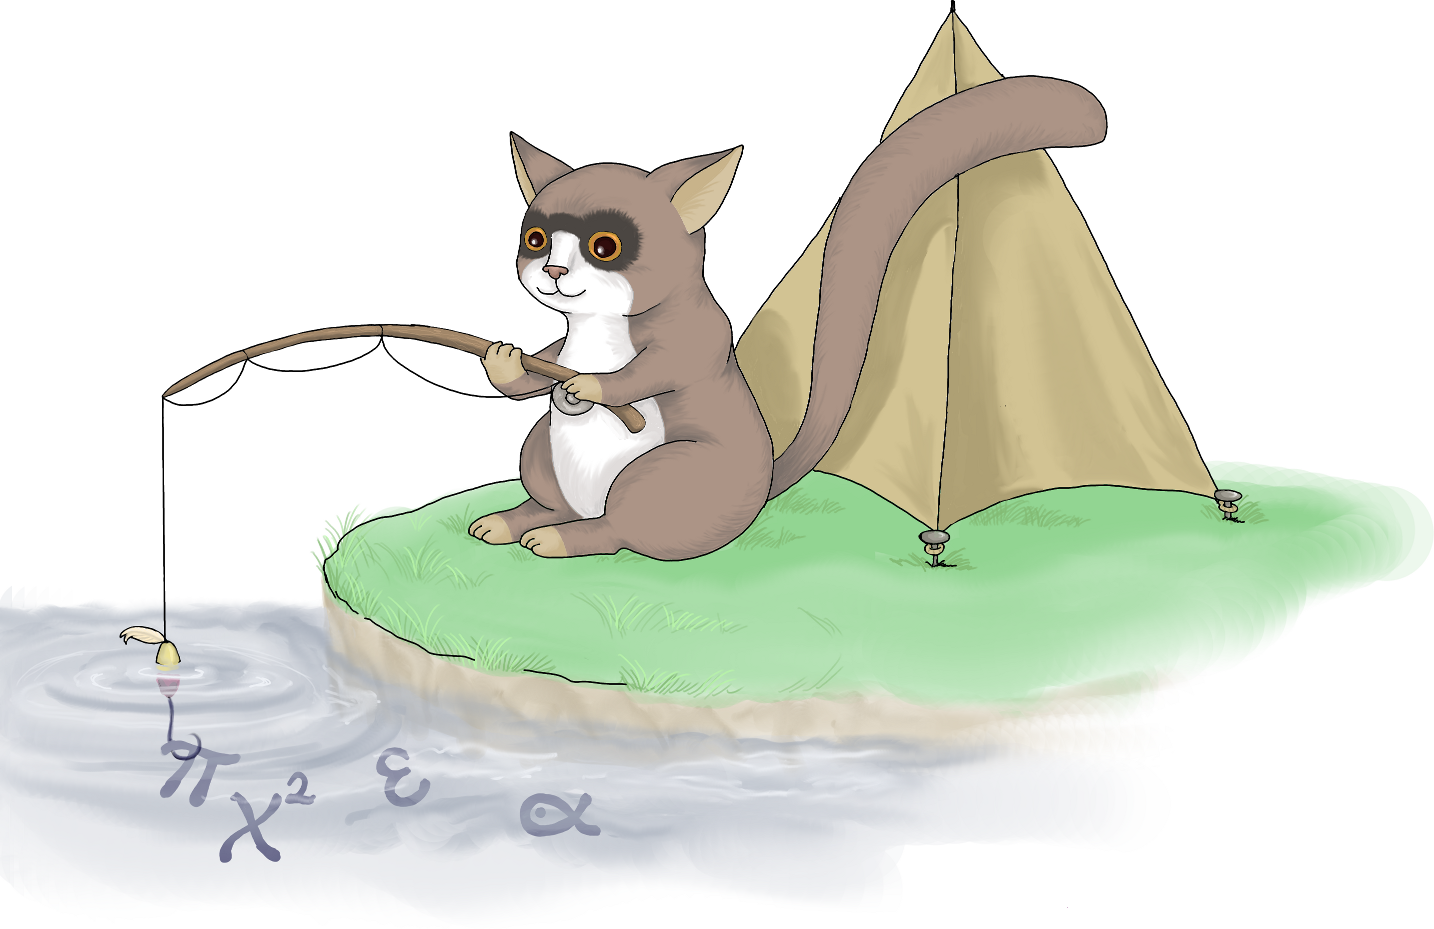
\includegraphics[scale=0.18]{campgregor}}}

\usepackage{framed}
\definecolor{shadecolor}{rgb}{.97,.97,.97}

\geometry{tmargin=1.5cm,bmargin=1.5cm,lmargin=2.0cm,rmargin=2.0cm}

\def\chopline#1;#2;#3;#4;#5;#6;#7;#8 \\{
  \def\vorname{#3}
  \def\nachname{#2}
  \def\strasse{#5}
  \def\plzort{#6}
 }
\newif\ifmore\moretrue

\begin{document}

\renewcommand{\betreff}{Mathecamp -- schön war's!}

\newread\quelle
 \openin\quelle=kinder.csv
 
 \loop
  \read\quelle to \zeile
  \ifeof\quelle
   \global\morefalse
  \else
   \expandafter\chopline\zeile\\

\renewcommand{\anschrift}{
      \vorname~\nachname \\
      \strasse \\
      \plzort \\
      \ \\
      \ \\}

\makeletterhead{}

%\begin{picture}(0,0)
%  \put(7.0,-19.0){%
%    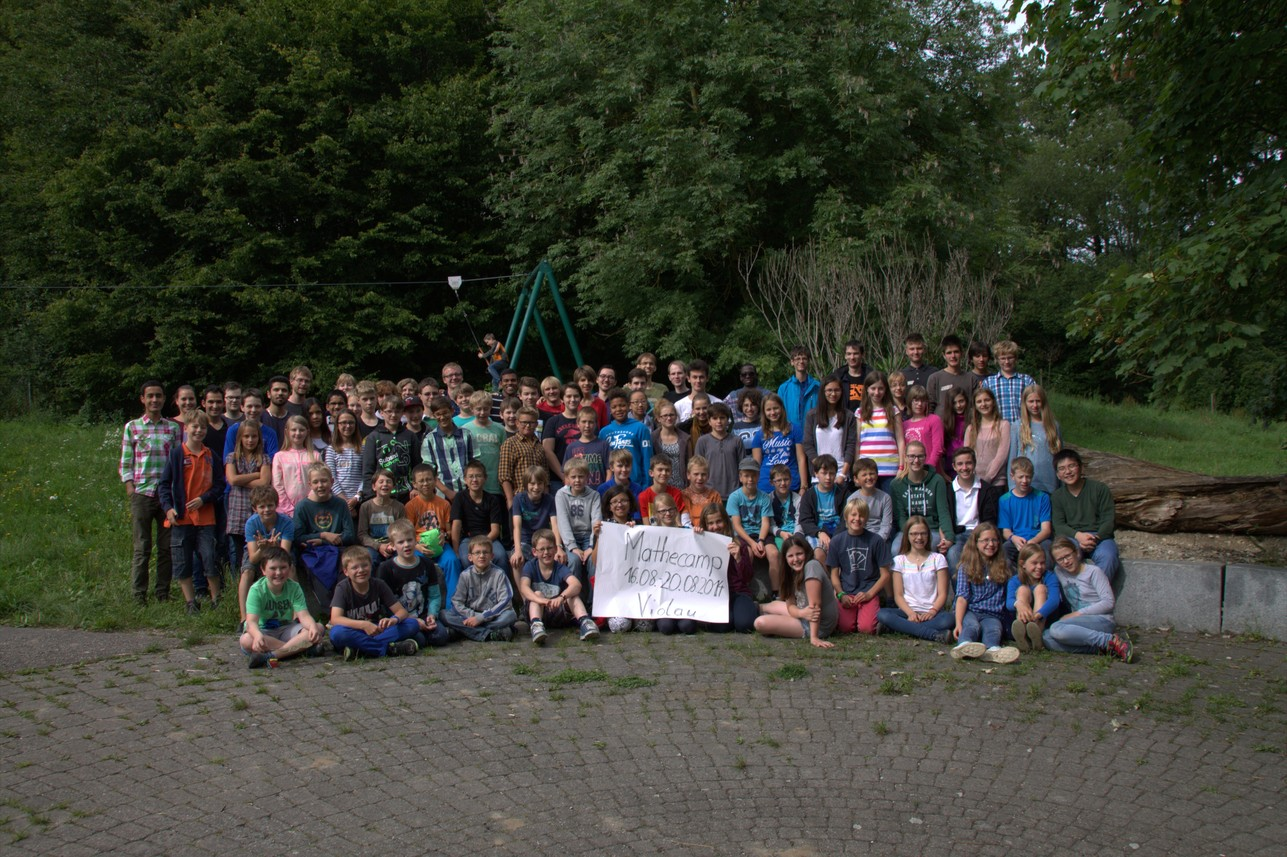
\includegraphics[scale=0.2]{gruppenfoto}
%  }
%\end{picture}
\vspace{-2em}

Liebe Schülerinnen und Schüler, liebe Eltern,

hoffentlich hattet ihr nach dem Mathecamp noch schöne Ferien und jetzt einen
guten Start in das neue Schuljahr! Wir hoffen, dass ihr nicht nur die
mathematischen Themen interessant fandet, sondern ihr auch rundherum viel
Spaß hattet. Uns hat das Camp mit euch sehr viel Freude bereitet.

Eine Fotogalerie gibt es unter \textsf{http:/\!/tiny.cc/mathe}
(Benutzername \textsf{mathe}, Passwort \textsf{fibonacci}).

\begin{center}
  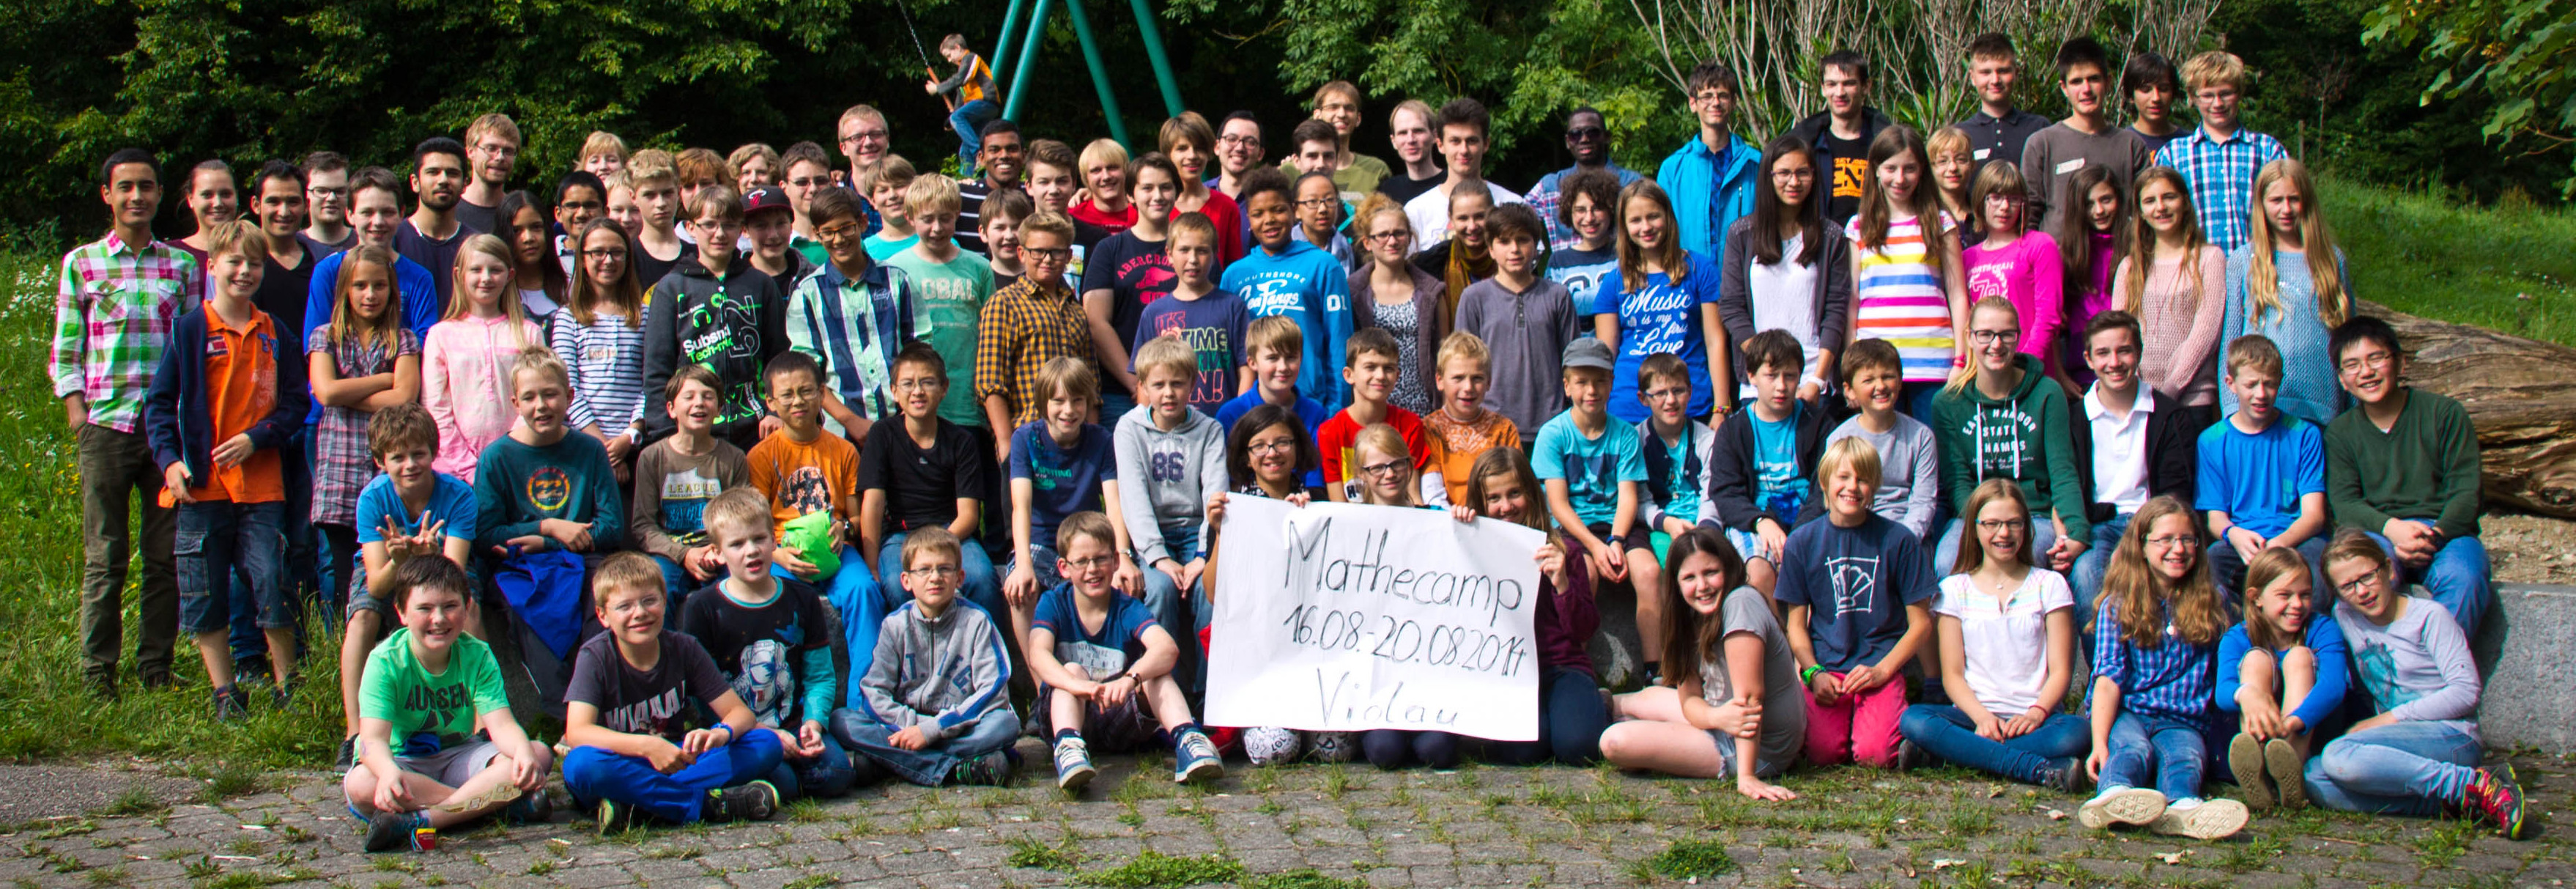
\includegraphics[scale=1.2]{gruppenfoto-ausschnitt}
\end{center}

Nächstes Jahr werden wir das Camp wieder veranstalten -- euren Rückmeldungen
entsprechend dann voraussichtlich sieben statt nur fünf Tage. Diesbezüglich
werden wir euch rechtzeitig informieren. Natürlich hören wir auch gerne
konstruktive Kritik, damit wir das nächste Mathecamp noch besser
machen können. Schickt uns einfach eine Mail an
\textsf{mathezirkel@math.uni-augsburg.de} oder ruft an (0821/598-5601).

Wir bedanken uns herzlich bei \emph{Bündnis für Augsburg}, dem
\emph{Mathematisch-Physikalischen Verein} und den Professorinnen und
Professoren der Lehrstühle für \emph{Algebra und Zahlentheorie},
\emph{Angewandte Analysis} und \emph{Nichtlineare Analysis} des Instituts für
Mathematik für ihre Unterstützung.
Ganz besonderer Dank gebührt einem Professor des
Lehrstuhls für \emph{Analysis und Geometrie}.

Nicht zuletzt bedanken wir uns bei Ihnen, liebe Eltern, für die zahlreichen
Spenden. Das wissen wir sehr zu schätzen.
Wenn Sie Kontakte zu Firmen oder Stiftungen haben, die potenziell gewillt
wären, das Mathecamp im nächsten Jahr zu unterstützen, freuen wir uns über
geeignete Hinweise.

Wir wünschen euch viel Spaß und Erfolg im neuen Schuljahr und würden uns
sehr freuen, euch bei der Eröffnungsveranstaltung des Matheschülerzirkels am
18.~Oktober oder spätestens beim Mathecamp im nächsten Jahr wiederzusehen!
\emph{Euer Mathecamp-Team}

{\small Meru Alagalingam, Martin Baur, Ingo Blechschmidt, Tim Dafler, Philipp Düren,
Alexander Engel, Kathrin Helmsauer,
Christian Hübschmann, Jil Hümmer, Sven Prüfer,
Lisa Reischmann, Peter Uebele}

\newpage

\fi
\ifmore\repeat

\closein\quelle

\end{document}
